\documentclass[10pt,a4paper]{article}
\usepackage{needspace}
\usepackage[nobottomtitles]{titlesec}
\usepackage{multicol}
\usepackage{xcolor}
\usepackage{fp}
\usepackage{xfp}
\usepackage{enumitem}
\usepackage{WriteOnGrid}
\usepackage{frcursive}
\usepackage{csvsimple}%
\usepackage[francais,bloc]{automultiplechoice}

\FPseed=10

\baremeDefautS{e=0,v=0,b=1,m=-.1}
\baremeDefautM{e=0,v=0,b=.5,m=-.1}

\graphicspath{ {./images/} }

\newenvironment{reponsesd}{
    \begin{multicols}{2}
    \begin{reponses} }{
    \end{reponses}
    \end{multicols}
}

\setlength{\columnseprule}{1pt}
\def\columnseprulecolor{\color{lightgray}}%

\let\oexplain\explain
\renewcommand{\explain}[1]{\oexplain{\textcolor{red}{#1}}}

\titleformat{\section}
  {\centering\hrule\vspace{2mm}}
  {\thesection}
  {1em}
  {}
  [\vspace{1mm}\hrule]

\titleformat{\subsection}
  {\em}
  {\thesubsection}
  {1em}
  {}

\newcommand{\sujet}{
\exemplaire{1}{%

\AMCsetFoot{\niveau{} \classe{} -- \prenom{}~\nom{} -- \thepage}

%%% debut de l'en-tête des copies :
\begin{center}
\vfill
\noindent{\large \bf Classe de \niveau{}°\classe{}}

\vspace*{3mm}

{\Large\bf Évaluation de compétences (non notée) STL - Physique-Chime 15/10/2025}

\vfill
\namefield{\noindent{}\fbox{\vspace*{3mm}
         \Huge\bf\prenom{}~\nom{}\normalsize{}%
         \vspace*{3mm}
      }}
\end{center}
\vfill

\begin{center}
\textbf{Durée : 30 minutes.}
\vspace*{5mm}

  Aucun document n'est autorisé.
  L'usage de la calculatrice est interdit.

  Les questions faisant apparaitre le symbole \multiSymbole{} peuvent
  présenter une ou plusieurs bonnes réponses. Les autres ont
  une unique bonne réponse.

  {\color{white} Des points négatifs seront affectés aux mauvaises réponses.}
  \vspace*{5mm}

  \textbf{IMPORTANT: Utilisez un crayon de papier bien noir pour cocher les cases, et une gomme pour effacer délicatement en cas d'erreur. Ne raturez pas les cases. Si vous effacez le pourtour de la case, ne le redessinez pas!}

  \vspace*{5mm}

  Ne pas faire comme ceci (pas centré, trop pâle, raturé):\\
  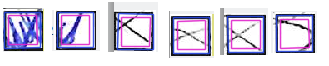
\includegraphics[width=4cm]{checkbox_bad.png}

  Mais comme cela (bien centré, bien foncé):\\
  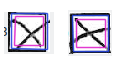
\includegraphics[width=2cm]{checkbox_good.png}

  Si vous faites une erreur et que vous ne pouvez effacer, raturez la case bien ostensiblement.

\end{center}
\vspace{1ex}
\vfill
\pagebreak
%%% fin de l'en-tête

\restituegroupe{groupes}


\AMCassociation{\id}

	  } % End \exemplaire{1}{%
} % End \newcommand{\sujet}{


%%%%§§§§§§§§§§§§§§§§§§§§§§§§§§§§§§§§§
\newcommand{\allq}{}
\newcommand{\nball}[1]{#1}

\begin{document}
%%%Options
\AMCrandomseed{10}

\def\AMCformQuestion#1{{\sc Question #1 :}}

\setdefaultgroupmode{withoutreplacement}
%%% Fin Options

%%% elements

\element{meta}{
  \begin{question}{meta1}\QuestionIndicative
    Pensez-vous poursuivre vos études dans un domaine lié à la physique, la chimie ou la biologie~?
    \begin{reponses}[o]
      \bonne{Oui}
      \bonne{Peut-être}
      \bonne{Ne sait pas}
      \bonne{Probablement pas}
      \bonne{Non}
    \end{reponses}
    \explain{C'est votre choix.}
  \end{question}

  \begin{question}{meta2}\QuestionIndicative
    Si oui, plutôt dans quel domaine (et sinon, quoi)~?
    \begin{reponses}[o]
      \bonne{Physique}
      \bonne{Chimie}
      \bonne{Biologie}
      \bonne{Autre, précisez: }
    \end{reponses}
    \explain{C'est votre choix.}
  \end{question}

  \begin{question}{meta3}\QuestionIndicative
    Que vous souhaitiez en faire votre métier ou non, aimez-vous la physique, la chimie ou la biologie~?
    \begin{reponses}[o]
      \bonne{Oui}
      \bonne{Un peu}
      \bonne{Ne sait pas}
      \bonne{Pas trop}
      \bonne{Non}
    \end{reponses}
    \explain{C'est votre choix.}
  \end{question}

  \begin{questionmult}{meta4}\QuestionIndicative
    Que préférez-vous (plusieurs choix possibles)~?
    \begin{reponses}[o]
      \bonne{Physique}
      \bonne{Chimie}
      \bonne{Biologie}
      \bonne{Mathématiques}
      \bonne{Autre, précisez: }
    \end{reponses}
    \explain{C'est votre choix.}
  \end{questionmult}

} % End \element{meta}{

\element{strspc}{
  \begin{questionmult}{strspc1}
    Une molécule est dite chirale si~:
    \begin{reponses}
      \mauvaise{ses atomes sont alignés}
      \mauvaise{elle est superposable à son image dans un miroir}
      \mauvaise{ses énantiomères sont diastéréoisométriques}
      \bonne{elle n'est pas superposable à son image dans un miroir}
    \end{reponses}
    \explain{un composé est dit chiral s'il n'est pas superposable à son 
    image dans un miroir plan.}
  \end{questionmult}

  \begin{questionmult}{strspc2}
    La conformation d'une molécule se défini par~:
    \begin{reponses}
      \mauvaise{ses caractéristiques isomérique}
      \mauvaise{son respect des spécifications de son espèce chimique}
      \mauvaise{la qualité de son image dans un miroir plan}
      \bonne{les arangement des atomes tournant autour de liaisons simples}
    \end{reponses}
    \explain{La conformation d'une molécule correspond à l'orientation des atomes autour
    de liaisons simples. Celle-ci pouvant la plupart du temps tourner librement, 
    le même composé chimique peut passer de une à l'autre facilement.}
  \end{questionmult}
  
  \begin{questionmult}{strspc3}
    La configuration d'une molécule est~:
    \begin{reponses}
      \mauvaise{la version de système d'exploitation installé par défaut}
      \mauvaise{les arangement des atomes tournant autour de liaisons simples}
      \mauvaise{son image dans un miroir plan}
      \bonne{la disposition de ses atomes dans l'espace indépendamment des rotations
      autour des liaisons simples}
    \end{reponses}
    \explain{La configuration d'une molécule correspond à l'orientation des atomes dans l'espace,
    indépendamment des rotations autour des liaisons simples. Pour changer de configuration,
    il faut casser des liaisons pour en reformer d'autres.}
  \end{questionmult}

  \begin {questionmult}{strspc4}
    Deux molécules sont des stéréo-isomères chimiques, si~:
    \begin{reponses}
      \mauvaise{elles ont une formule brute différente mais les mêmes propriétés chimiques}
      \mauvaise{elles ont la même conformation}
      \mauvaise{elles ont la meme configuration mais une formule semi-développée differente}
      \bonne{elles ont même formule semi-développée mais une configuration différente}
    \end{reponses}
    \explain{Les stéroisomères chimiques sont des molécules ayant la même formule
    semi-développée mais une conformation ou une configuration différente.}
  \end {questionmult}

  \begin {questionmult}{strspc5}
    Deux molécules sont des énantiomères chimiques, si~:
    \begin{reponses}
      \mauvaise{elles ont même formule semi-développée mais ne sont pas images de l'une de l'autre dans un miroir plan}
      \mauvaise{elles ont la même mère}
      \mauvaise{la rotation de leur image dans un miroir dessine une ligne de symétrie}
      \bonne{elles sont images de l'une de l'autre dans un miroir plan}
    \end{reponses}
    \explain{Les enantiomères chimiques sont des molécules qui sont images de l'une de
    l'autre dans un miroir plan.}
  \end {questionmult}

  \begin {questionmult}{strspc6}
    Deux molécules sont des diastéréoisométriques chimiques, si~:
    \begin{reponses}
      \mauvaise{elles ont une formule brute differente mais sont images de l'une de l'autre dans un miroir plan}
      \mauvaise{elles sont très très malades}
      \mauvaise{elles sont images de l'une de l'autre dans un miroir plan}
      \bonne{elles ont même formule semi-développée mais ne sont pas images de l'une de l'autre dans un miroir plan}
    \end{reponses}
    \explain{Les diastéréoisométriques .}
  \end {questionmult}
} % fin de l'element strspc
%\setgroupmode{strspc}{withoutreplacement}
%%%% fin des elements

\element{groupes}{
\section{Méta}
\begin{multicols}{2}
\restituegroupe[1]{meta}
\end{multicols}

\section{Structures spatiales des espèces chimiques}
\begin{multicols}{2}
\restituegroupe{strspc}
\end{multicols}
\AMCcleardoublepage
}

\csvreader[head to column names]{liste.csv}{}{\sujet}

\end{document}
